\documentclass[ngerman]{schoolPres}

\usepackage[
  type={CC},
  modifier={by-sa},
  version={4.0},
  imagemodifier={-eu-80x15},
]{doclicense}

% \setbeameroption{show only notes} % Only notes
% \setbeameroption{show notes on second screen=right} % Both

\setbeamertemplate{section in toc}{%
  \leavevmode%
  \hspace{.42\textwidth}
  \llap{%
    \hbox to2.25ex{\hfil\usebeamercolor[fg]{background}{\tikz[baseline=-.75ex]{\fill (0,0) circle (.5ex)}\hfil}}
  }%
  \kern1.25ex\inserttocsection\par%
}

\newcommand{\FramedSection}[1]{
  \section{{#1}}%
  \begin{frame}%
    \vfill\begin{beamercolorbox}[sep=12pt, center]{title}%
      \usebeamerfont{title}{#1}\par%
    \end{beamercolorbox}\vfill%
  \end{frame}%
}

\usepackage[backend=biber, style=numeric, sorting=none]{biblatex}
\addbibresource{ref.bib}
\renewcommand*{\bibfont}{\scriptsize}

% \usepackage{todonotes}

\date{2023-02-21}
\author{C. Badermann}
\title{Die Speicherkarte}
\subtitle{Kompakter Speicher mit großem Potenzial; der vertraute Gefährte der Datenaggregation}

\begin{document}

  \section{Prolog}%
  \subsection{Titelfolie}%
  \begin{frame}
    \titlepage

    \begin{center}
      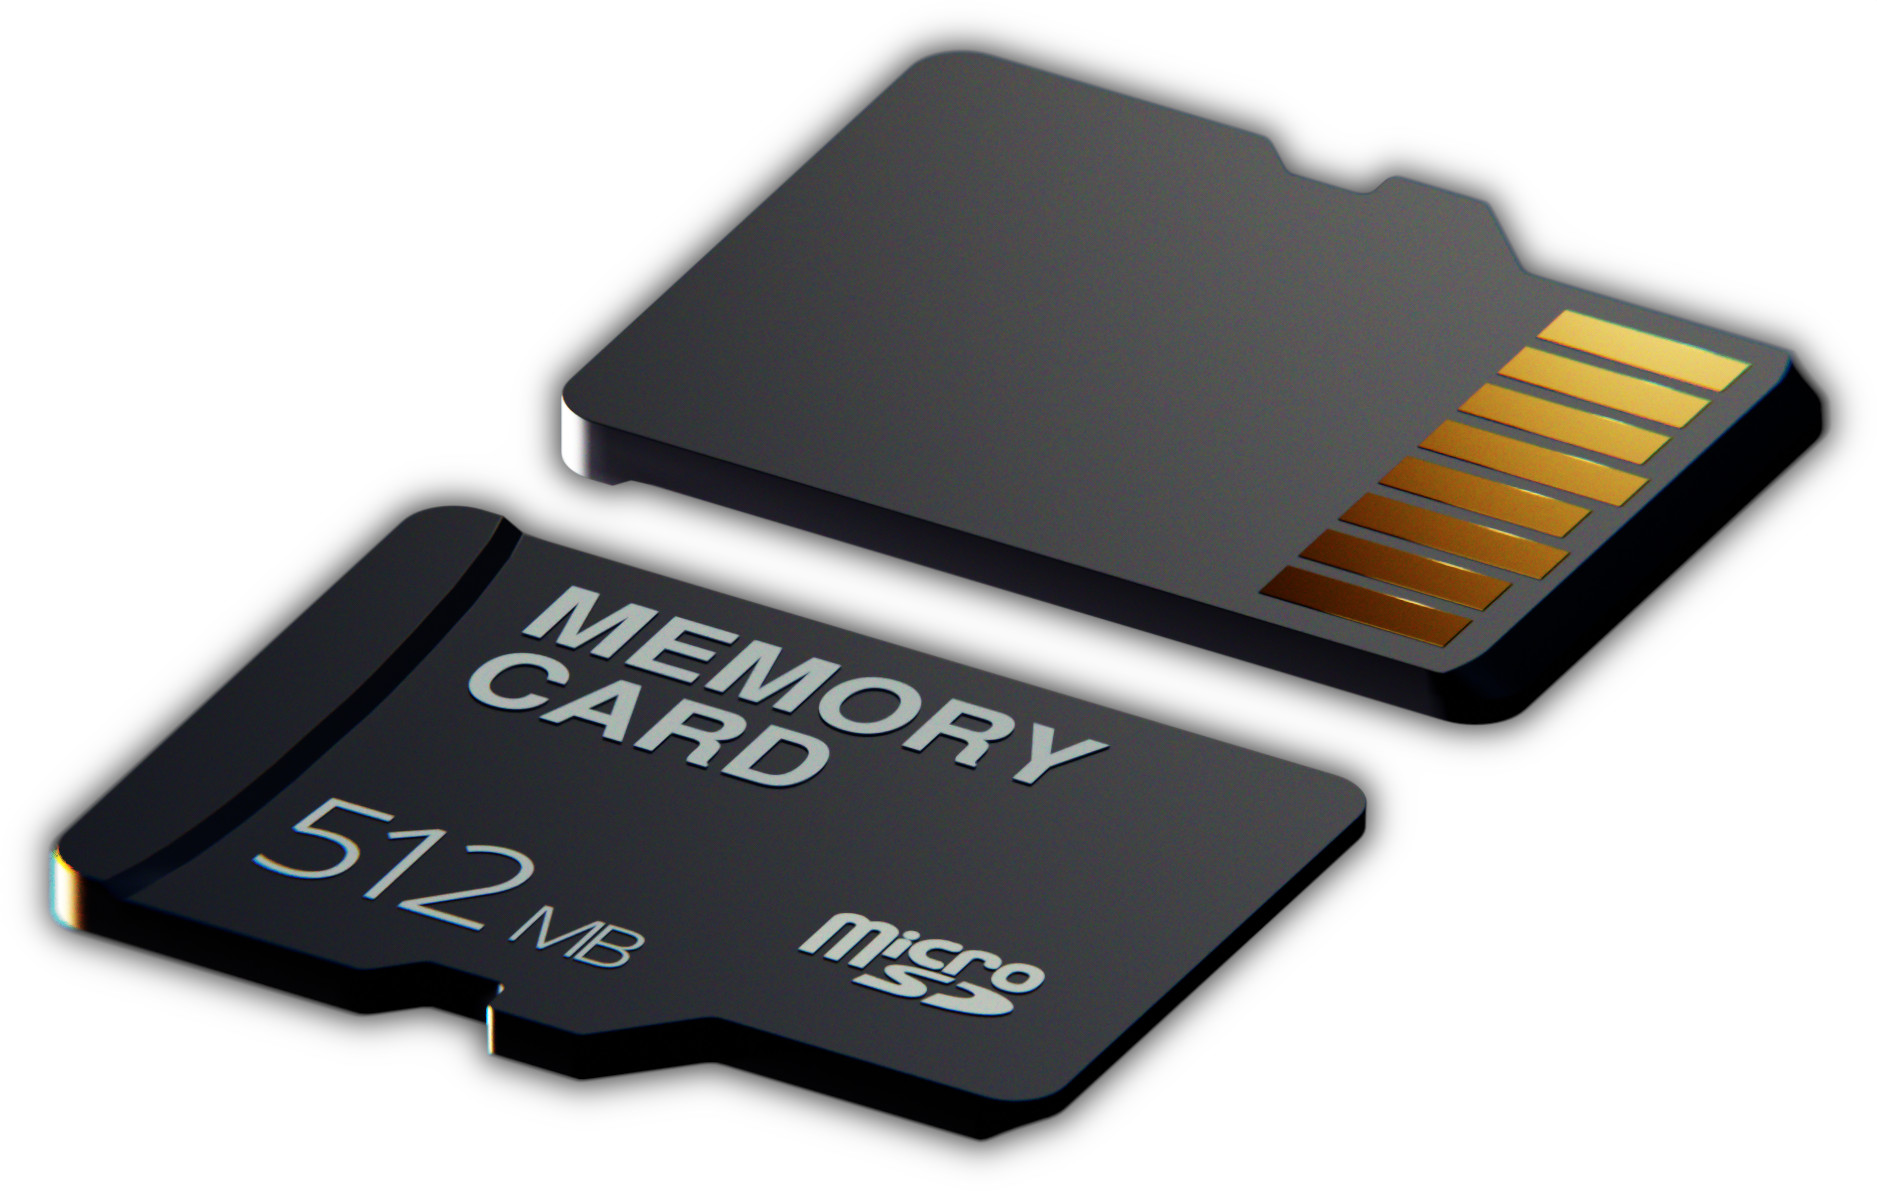
\includegraphics[height=8em]{media/title_edit.jpg}
    \end{center}
  \end{frame}

  \subsection{Inhaltsverzeichnis}%
  \begin{frame}
      \tableofcontents[hideallsubsections]

    \note{
      - Motivation \& Einleitung der MicroSD-Karte\\
      - Hardware-Aspekt\\
      - Software-Lösungen (ordnungsgemäßen Formatierung, Bibliotheken und deren Funktionen)\\
      - Beispielprojekt (Konstruktion nach Beschreibung, Software Design \& Programmierung, Datenanalyse)
    }
  \end{frame}

  \FramedSection{Die SD-Karte}%
  \subsection{Motivation}%
  \begin{frame}<1>[label=motivation]
    \usebeamercolor[fg]{structure}
    \only<2>{
      \begin{center}
        \textbf{Zur Erinnerung:}
      \end{center}
    }
    \usebeamercolor[fg]{normal text}

    \only<1>{\textbf{Szenario:}\\}
    Mithilfe der Arduino Plattform soll eine Wetterstation konstruiert werden. Gemessen werden Temperatur, Luftfeuchtigkeit und Luftdruck, mithilfe der \enquote{\texttt{HDC100x}} und \enquote{\texttt{BMP280}} Sensormodule.
    Zur Auswertung, sollen die über einen längeren Zeitraum gemessenen Datenpunkte aggregiert und auf einen persönlichen Computer übertragen werden\cite{EnergyLab-Wettermessstation}.\\~\\
    \only<1>{\note{
      Szenario:\\
      Wettermessstation, Aggregation auf Speichermedium, Auswertung am PC.\\~\\
    }}

    \only<1>{\textbf{Erwünschte Fähigkeiten des Speicher- \& Übertragungsmedium:}
    \begin{itemize}
      \item Nichtflüchtige \& alleinstehende Speicherung
      \item Einfacher Transfer von eingelesenen Daten auf andere Systeme
      \item Großes Speichervolumen
    \end{itemize}
    \note{
      - Nichtflüchtigkeit! (RAM / ROM)\\
      - Alleinstehend (ohne externe Systeme)
    }}
  \end{frame}

  \subsection{SD \& SDA}%
  \begin{frame}
    Ein geeignetes Speichermedium für dieses Szenario ist die microSD-Karte.
    Diese ist das physisch kleinste Mitglied der Familie der SD-Karten, \href{https://de.wikipedia.org/wiki/Flash-Speicher}{Flash-EEPROM} nach Standard der \enquote{SD Association}.\\~\\

    \textbf{Qualitäten:}
    \begin{itemize}
      \item Kostengünstig
      \item Allgegenwärtig
      \item Kompakter Formfaktor
      \item Simple SPI Schnittstelle
      \item Müheloses Einführen, Entfernen
      \item Verfügbarkeit von Anschlüssen für den Arduino und andere Systeme
    \end{itemize}

    \note {
      microSD-Karten sind cool! Yay\\

      Viele tolle Eigenschaften...
    }

    \blfootnote{\citeauthor{sd-overview} -- \enquote{\citetitle{sd-overview}}\cite{sd-overview}.}
  \end{frame}

  \begin{frame}
    SD-Karten ermöglichen die Nichtflüchtige Speicherung von Daten.
    Diese sind als Dateien in einem Ordersystem organisiert.\\~\\

    \textbf{Obacht:}
    \begin{itemize}
      \item \enquote{\texttt{SD.h}} unterstützt nur bestimmte Karten\cite{sd-lib}
      \item Flash-Speicher verfügt über endlich viele Schreibzyklen\cite{zhang2017flash,sd-lifespan}
      \item SD-Karten sind leicht zu verlegen und können ohne Weiteres entwendet werden
      \item Es gibt leistungsfähigeren Speicher
      \item SD ist ein proprietärer Standard\cite{sd-proprietary}
    \end{itemize}

    \note {
      Es gibt einiges zu beachten...
    }
  \end{frame}

  \FramedSection{Hardware}%
  \subsection{SD-Karten}%
  \begin{frame}
    \begin{columns}[c]
      \begin{column}{.6\linewidth}
        Die Hardware von (micro-) SD Karten ist durch einen Standard der \enquote{SD Association} festgelegt.
        Dieser Spezifiziert z.B.: Funktionsweise \& Dimensionen der Produkte, welche unter dem \emph{SD} Warenzeichen verkauft werden dürfen.\\~\\

        In miroSD-Karten sind Maße von etwa 11x15x1{mm}, sowie eine wohl definierte Schnittstelle zu erwarten.
        Eine Kerbe ermöglicht das Einrasten in Lesegeräte.\\~\\

        Im inneren der Karten sind unter anderem der Flash-Speicher, sowie ein Mikrocontroller zu finden.
        Letzterer stellt nutzerfreundliche Protokolle zur strukturierten Nutzung des Speichers zur Verfügung.
      \end{column}
      \begin{column}{.4\linewidth}
        \begin{figure}[!ht]
          \centering
          \begin{subfigure}{.65\linewidth}
            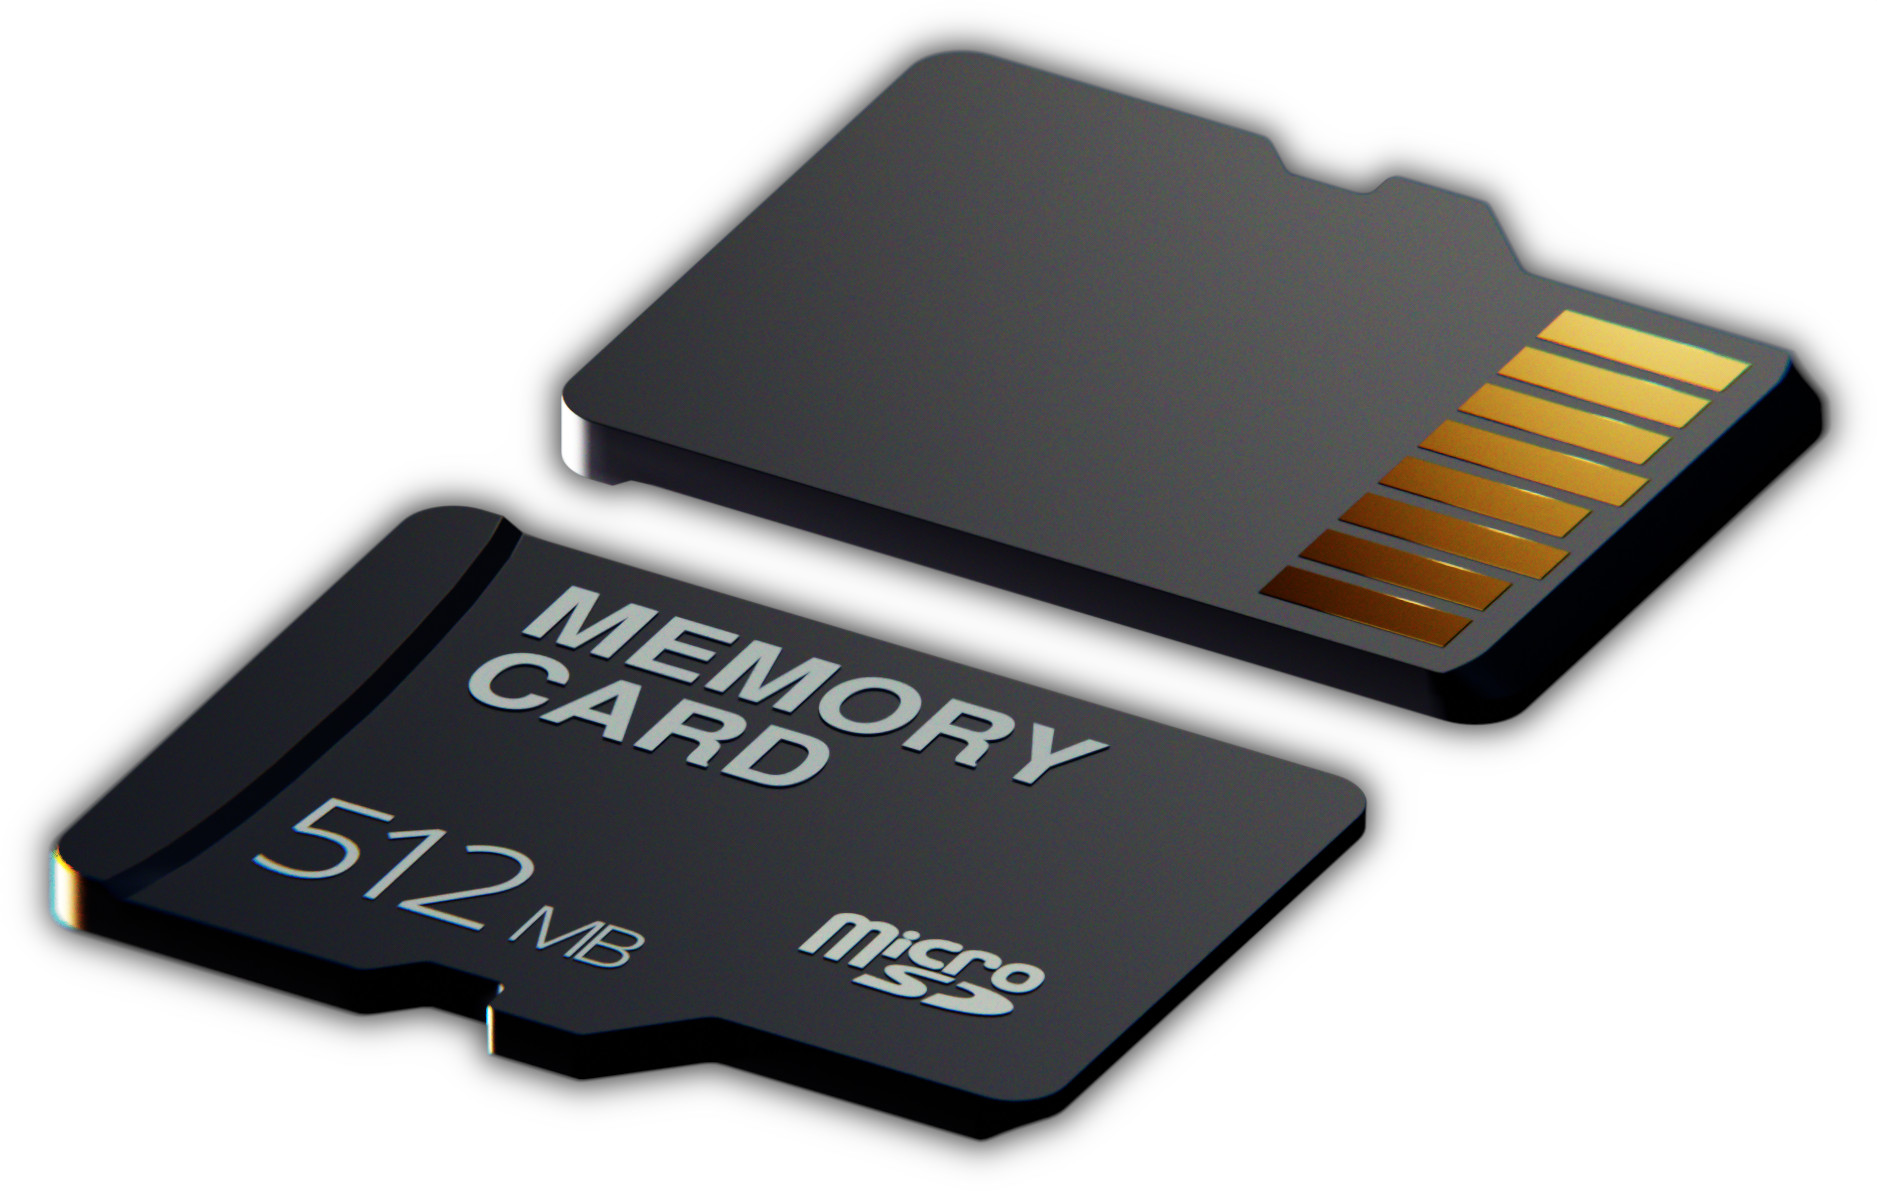
\includegraphics[width=\linewidth]{media/title_edit.jpg}
          \end{subfigure}\vspace{1em}

          \begin{subfigure}{.3\linewidth}
            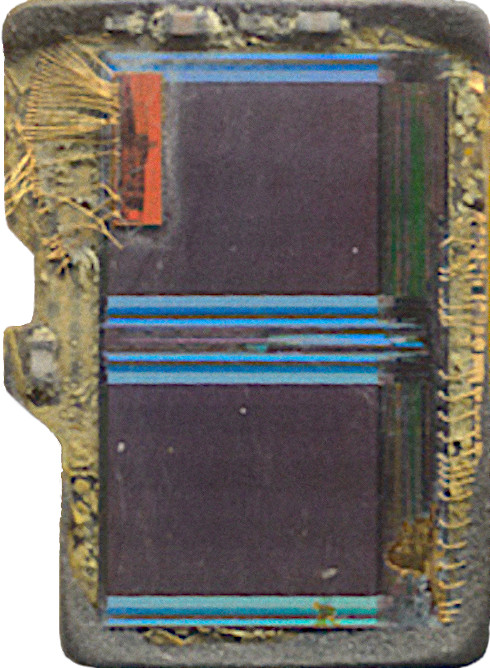
\includegraphics[width=\linewidth]{media/decapsulated-01.jpg}
            \caption{\tiny \href{https://commons.wikimedia.org/wiki/File:Decapsulated\_microSD\_memory\_card\_lineup-genuine,\_questionable,\_and\_fake-counterfeit.jpg}{Andrew Huang\\CC BY-SA 3.0}}
          \end{subfigure}\hspace{4em}
          \begin{subfigure}{.3\linewidth}
            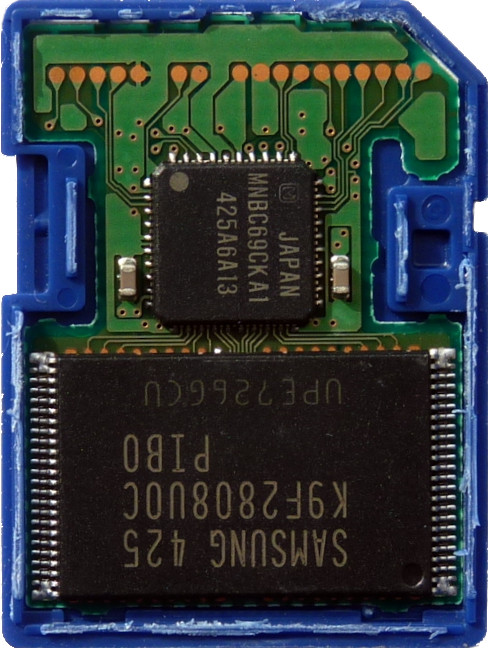
\includegraphics[width=\linewidth]{media/decapsulated-02.jpg}
            \caption{\tiny \href{https://commons.wikimedia.org/wiki/File:SDKarteoffen.jpg}{Fritz Jörn\\CC BY 3.0}}
          \end{subfigure}
        \end{figure}
      \end{column}
    \end{columns}

    \blfootnote{\citeauthor{sd-spec_physical-layer} -- \enquote{\citetitle{sd-spec_physical-layer}}\cite{sd-spec_physical-layer}.}
    \note {
      Hardware definiert durch spec der SDA; SD Trademark sichert ab.\\~\\

      Physische Beschreibung\\~\\

      Innenleben: Flash-Speicher \& Mikrocontroller.\\
      nutzerfreundliches Protokoll
    }
  \end{frame}

  \subsection{Interfaces}%
  \begin{frame}
    Zur Verbindung des Arduino mit SD-Karten gibt es verschiedene Schnittstellen.
    Häufig sind Shields mit microSD Anschluss und Breakout-Boards,
    welche die Kontakte der SD-Karte zur Verfügung stellen und ggf. die Stromstärke regulieren.
    Durch beide wird die Karte an den SPI-Bus des Arduino angehangen.\\~\\

    \begin{figure}[!ht]
      \centering
      \begin{subfigure}{.3\linewidth}
        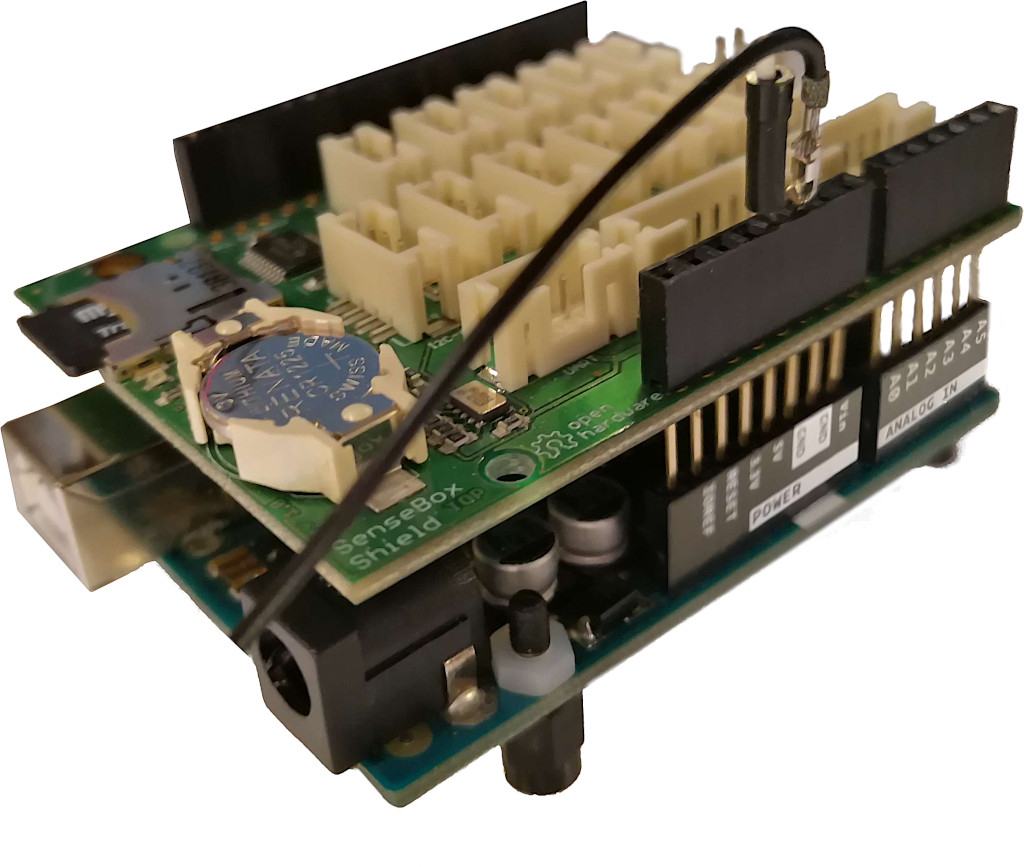
\includegraphics[width=\linewidth]{media/shield.jpg}
        \caption{\tiny Shield mit microSD Anschluss}
      \end{subfigure}\hspace{4em}
      \begin{subfigure}{.3\linewidth}
        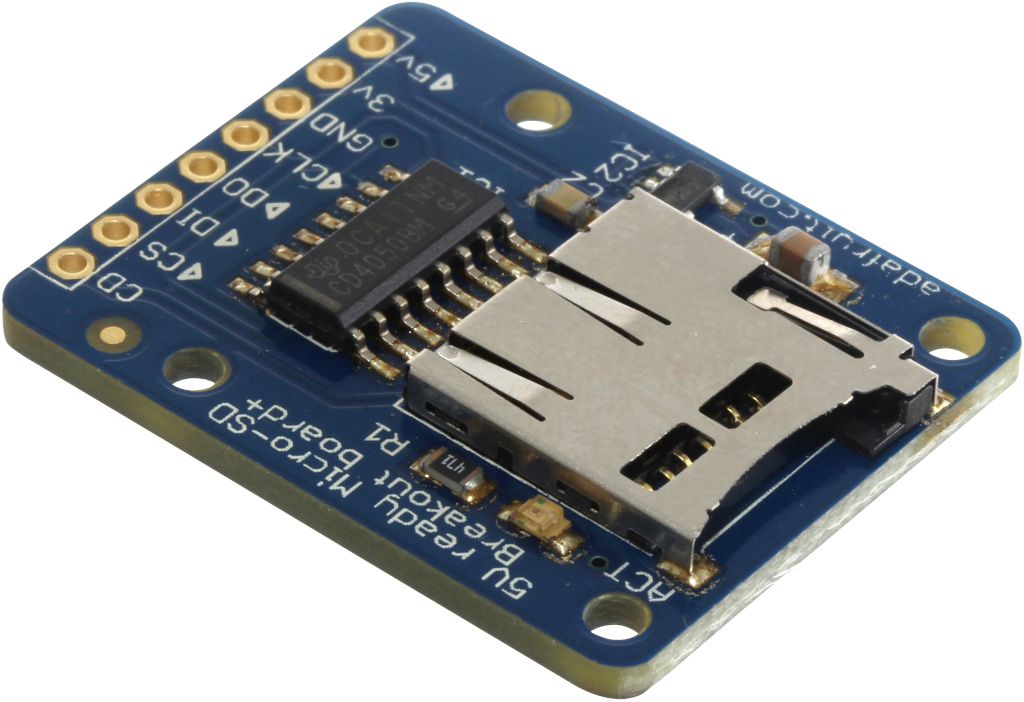
\includegraphics[width=\linewidth]{media/sd-breakout.jpg}
        \caption{\tiny microSD breakout board\\(\href{https://www.flickr.com/photos/snazzyguy/6234676208/}{oomlout, CC BY-SA 2.0})}
      \end{subfigure}
    \end{figure}

    \note {
      Schnittstellen: Shields \& Breakout-Boards.\\
      Beide per SPI-Bus.
    }
  \end{frame}

  \FramedSection{Software}%
  \subsection{SD-Karte}%
  \begin{frame}
    Für die Verwendung einer microSD-Karte mit dem Arduino, muss diese gegebenenfalls formatiert werden.
    Unterstützt werden MBR / DOS oder die kompatible GUID-Partitionstabelle mit FAT16 / FAT32 Dateisystemen\cite{sd-lib}.

    \vspace{2em}

    Nicht integrierte System nutzen häufig SD-Bus, UHS-II Bus, oder PCIe, anstelle von SPI.
    Dies erlaubt für Karten mit größeren Speichervolumen und höheren Transfergeschwindigkeiten.
    Für den Arduino ist dies insofern relevant, als diese nicht direkt verfügbar sind.
    Bestimmte Konfigurationen des SD Standards können nicht verwendet werden\cite{sd-spec_physical-layer}.

    \note {
      Speichermedium-Formatierung ist ggf. notwendig.\\
      SD-Bus Umstände.
    }
  \end{frame}

  \subsection{SD Library}%
  \begin{frame}
    Zur Verwendung von SD-Karten findet die SD Library Gebrauch.
    Sie kann über den Library Manager installiert, und als \enquote{\texttt{SD.h}} eingebunden werden.
    Zur Kommunikation über den SPI-Bus wird ebenfalls \enquote{\texttt{SPI.h}} benötigt.

    \note {
      SD Library (\texttt{SD.h} \& \texttt{SPI.h}); Installation in IDE 1.x \& 2.x.
    }

    \vfill
    \begin{figure}[!ht]
      \centering
      \begin{subfigure}{.75\linewidth}
        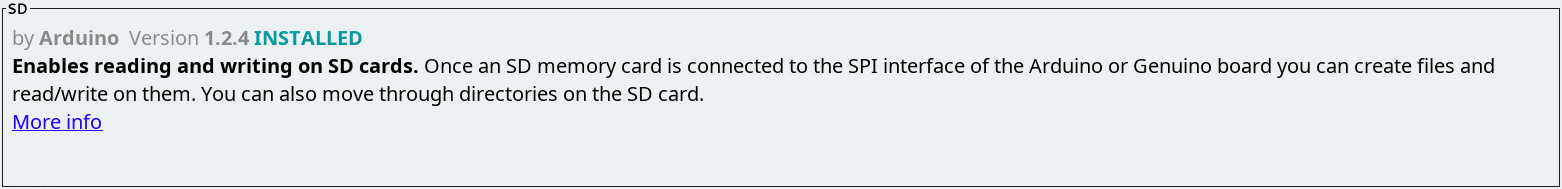
\includegraphics[width=\linewidth]{media/sd-lib.png}
        \caption{Arduino IDE 1.8}
      \end{subfigure}\hspace{1.5em}
      \begin{subfigure}{.2\linewidth}
        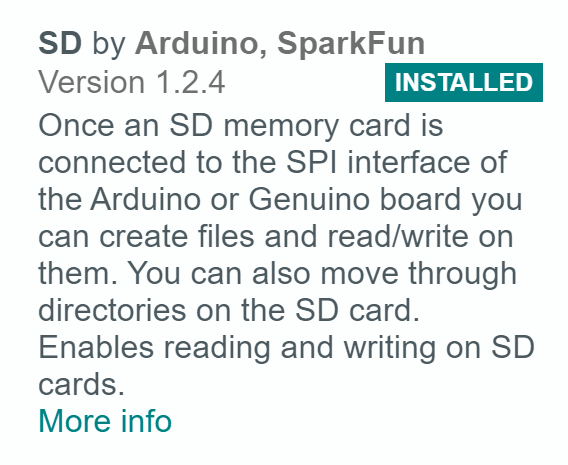
\includegraphics[width=\linewidth]{media/sd-lib-ide2.png}
        \caption{Arduino IDE 2.0}
      \end{subfigure}
    \end{figure}
    \begin{center}
    \end{center}
  \end{frame}

  \begin{frame}[fragile]
    Nach Inklusion von \texttt{SPI.h} \& \texttt{SD.h} kann die programmatische Verwendung der SD-Karte beginnen.\\~\\

    Um die SPI-Verbindung herzustellen, wird die Funktion \enquote{\texttt{SD.begin(int cs)}} verwendet.
    Ihr Argument, \texttt{cs}, ist der \enquote{Chip-Select Pin} der SPI-Verbindung.
    \enquote{\texttt{SD.begin()}} liefert einen Boolean. Wahr / 1 bei Erfolg, Falsch / 0 bei Versagen.
    Dies kann mit einer If-Abfrage abgefangen werden, um den Programmfluss zu ändern, und ggf. den Nutzer zu informieren.

    \note {
      Inklusion der Header, Herstellung der SPI-Verbindung (Error Handling).
    }

    \lstinputlisting{./media/sketch/sd-setup.ino}
  \end{frame}

  \begin{frame}[fragile]
    \only<1> {
      Dateien sind die idiomatischen Container für Daten.\\
      Um sie zum Lesen und oder Schreiben zu öffnen, wird \enquote{\texttt{SD.open(dateipfad, modus)}} verwendet.
      Dies liefert das \texttt{File} Objekt, welches für weitere Operationen auf die Datei benötigt wird.

      \note {
        Dateien als Container.\\
        Öffnung dieser \& \texttt{File} Objekt.
      }
    }

    \only<2> {
      Modi beschreiben welche Aktionen auf die Datei ausgeführt werden können, z.B.: \texttt{File\_READ} \& \texttt{FILE\_WRITE}.
      Diese setzen sich ggf. aus weiteren Attributen zusammen. \texttt{File\_WRITE = (O\_READ | O\_WRITE | O\_CREAT | O\_APPEND)}.
      Es erlaubt demnach das Lesen, Schreiben, sowie Erstellen von Dateien, falls diese nicht bereits existieren. Es schreibt ans Dateiende.
      Diese Attribute können auch eigens gesetzt oder entfernt werden.

      \note {
        Öffungs-Modi und deren Funktion.
      }
    }

    \only<3> {
      Um Inhalte in Dateien zu schreiben, werden die bekannten \texttt{print()} Befehle auf das \texttt{File} Objekt angewandt.
      \texttt{write()} kann verwendet werden, um Binärdaten zu schreiben. \texttt{read()} ermöglicht das Lesen aus Dateien.

      \note {
        Schreiben und Lesen von Daten.
      }
    }

    ~\\
    \lstinputlisting{./media/sketch/sd-file.ino}
  \end{frame}

  \begin{frame}
    Die Bearbeitung des Dateisystems per \enquote{\texttt{SD.h}} ist durch die Funktionen \texttt{open}, \texttt{mkdir()}, \texttt{rmdir()}, \texttt{remove()} möglich.\\~\\

    Durch Abfragen wie \texttt{exists()}, \texttt{isDirectory()}, \texttt{name()}, können existierende Strukturen ertastet werden.\\~\\

    Per \texttt{open()}, \texttt{openNextFile()}, \texttt{rewindDirectory()} ist das Dateisystem zu navigieren. Beide \enquote{\texttt{open}} Funktionen sind ebenfalls für Ordern geeignet.

    \note {
      Dateisystemmanagement\\~\\

      Ertasten des Dateisystems\\~\\

      Navigierung des Dateisystems
    }
  \end{frame}

  \begin{frame}
    \textbf{Obacht:}\\~\\

    Das \texttt{File} Objekt erbt von \texttt{Stream} (Wie auch \texttt{Serial}) und ist somit gepuffert.
    Änderungen werden nicht direkt, sondern erst bei \texttt{flush} Ereignissen geschrieben.
    Dies geschieht z.B.: durch die \texttt{flush()} Funktion oder das Schließen einer Datei.
    Wird nicht geflushed, können Änderungen verloren gehen.\\~\\

    Versionsbedingt ist ggf. nur eine Datei an einem Zeitpunkt zu öffnen. Auch das mehrfache Öffnen derselben Datei ist davon betroffen. Das Schließen von Dateien sollte somit nicht vergessen werden.\\~\\

    Unterstützt sind lediglich \href{https://de.wikipedia.org/wiki/8.3}{8.3 Dateinamen} in Großbuchstaben\cite{sd-lib}.\\~\\

    (Gegensätzlich zum \enquote{\texttt{c}} \texttt{FILE}, wird das \texttt{File} Objekt der SD Library bis auf den ersten Buchstaben kleingeschrieben.)

    \note {
      \textbf{Zu beachten:}\\~\\

      \hspace{2em}File muss geflushed werden. Sonst können daten verloren gehen :/\\~\\

      \hspace{2em}\enquote{\texttt{SD.h}} kann ggf. nur eine Datei öffnen.\\~\\

      \hspace{2em}8.3 Dateinamen \& Diskrepanz zur Schreibweise des c \texttt{FILE} Objekt.
    }
  \end{frame}

  \FramedSection{Beispiel Projekt}%
  \hypertarget{sec:project}{}
  \subsection{Rückblick, Projektbeschreibung}%
  \againframe<2>{motivation}

  \subsection{Konstruktion}%
  \begin{frame}
    \begin{columns}[c]
      \begin{column}{.5\linewidth}
        Auf dem Arduino ist das \enquote{senseBox Shield} montiert.
        Es stellt eine Echtzeituhr (\href{https://de.wikipedia.org/wiki/Echtzeituhr}{RTC}) und den microSD Anschluss bereit.\\~\\

        Die besagten \enquote{\texttt{HDC100x}} \& \enquote{\texttt{BMP280}} Sensormodule sind auf der Steckplatine montiert und mit dem SPI-Bus des Arduino verbunden.
      \end{column}
      \begin{column}{.5\linewidth}
        \centering
        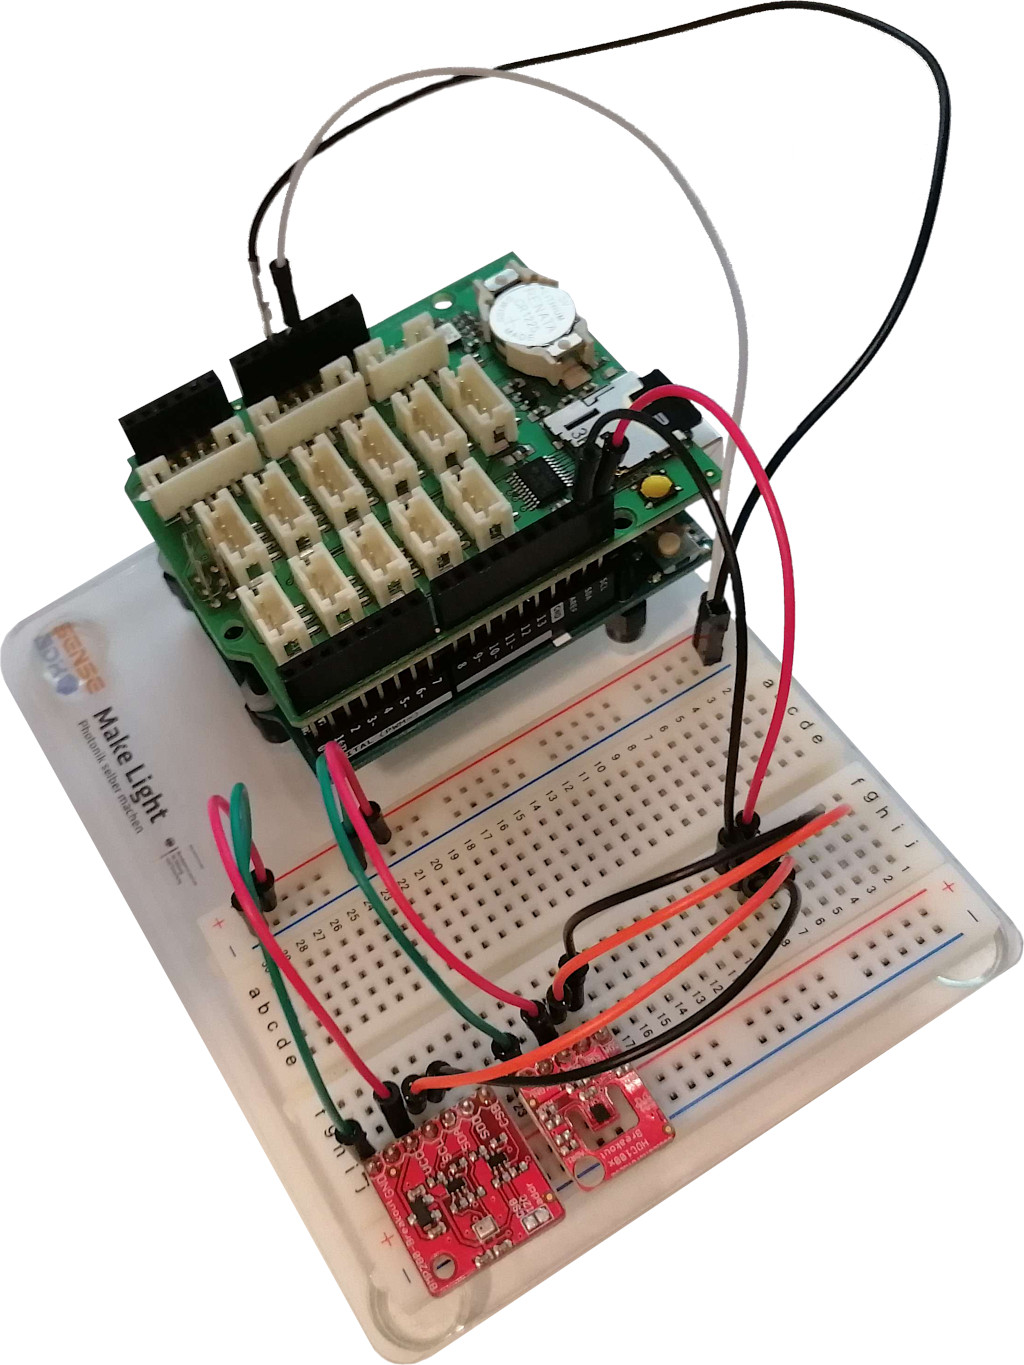
\includegraphics[height=.8\textheight]{media/board.jpg}
      \end{column}
    \end{columns}

    \note {
      Shield mit RTC und microSD Anschluss.\\~\\

      Sensoren am SPI-Bus.
    }
  \end{frame}

  \subsection{Speicherformate}%
  \begin{frame}
    Die Strukturierung der gesammelten Daten ist ein wichtiger Aspekt und bedeutend für die spätere Verarbeitung.
    Nutzerfreundlich sind textbasierte Formate.
    Um die Weiterverarbeitung zu erleichtern wird häufig strukturierter Text verwendet.
    Tabellen artige Strukturen sind gut in CSV darzustellen.
    Datenserialisierungssprachen eignen sich für komplexere Strukturen, welche Computerlesbar gespeichert werden
    sollen. Hier findet sich z.B.: XML, YAML, JSON.\\~\\

    \href{https://de.wikipedia.org/wiki/Bin\%C3\%A4rdatei}{Binärformate} können wesentlich platzsparender,
    und dadurch, aber auch durch die nicht notwendige Umwandlungen weniger zeitraubend sein.
    Das Einlesen dieser auf anderen Systemen kann jedoch deutlich komplizierter sein.
    Existierende Formate wie Protobuf, BSON können dies erleichtern.
    Individuelle Formate sind anspruchsvoller, aber nicht selten und bieten mehr Flexibilität.\\~\\

    Zu erwarten, sind ebenfalls menschliche oder technische Fehler.
    Von Daten, welche einen Wert haben, sollten stets unabhängige Sicherheitskopien existieren.
    Idealerweise auf mehreren Geräten oder sogar an mehreren Standorten\cite{chervenak-backup}.

    \note{
      Textbasierte Formate sind Nutzerfreundlich.\\
      Strukturierter Text ist cool für Computer.\\~\\

      Binärformate sind Kompakt, aber schwer einzulesen.\\
      Erschwertes Teilen durch fehlende Definition. (entropie ig?)\\
      Es gibt wohldefinierte Formate\\~\\

      Beispiel Sicherheitskopien:\\
      \hspace{2em} Jemand löscht aus Versehen den gesamten Datensatz des Projekts, beim Versuch diesen auszuwerten.
    }
  \end{frame}

  \begin{frame}[fragile]
    Da eine Reihe wiederholt gemessener Sensoren gut in einer Tabelle dargestellt werden kann, wurde das CSV (RFC 4180) Format gewählt\cite{rfc4180}.\\~\\

    Zeilen sind durch die Zeilenumbruchsequenz \enquote{\texttt{\textbackslash n}} oder \enquote{\texttt{\textbackslash r\textbackslash n}} getrennt.\\
    Datenfelder / Spalten durch das Komma \enquote{\texttt{,}}.\\~\\

    \lstinputlisting[caption={Beispiel CSV-Datei: (\href{https://de.wikipedia.org/w/index.php?title=CSV_(Dateiformat)\&oldid=229431469\#Beispiel}{Wikipedia -- CC BY-SA 3.0})}]{./media/sketch/csv.csv}

    \note {
      Erklärung CSV:\\~\\

      Tabellarische Darstellung. Trennung durch \enquote{\texttt{,}} \& newline.
    }
  \end{frame}

  \subsection{Programmierung}
  \begin{frame}[fragile]
    Alle verwendeten Sensormodule haben einfach zu verwendende Libraries und ähneln sich in ihren Funktionsweisen.
    Die Libraries werden eingebunden und die Sensoren definiert.\\
    \lstinputlisting{./media/sketch/include.ino}
    \note{
      Jeglicher Quelltext ist symbolisch zu Betrachten!\\
      Es sind nur Ausschnitte.\\~\\

      Einbindung der Libraries, Definition \& Initialisierung der Sensoren (immer ähnlich).
    }
  \end{frame}

  \begin{frame}[fragile]
    In \texttt{setup()} werden die SPI-Verbindungen initialisiert.\\
    \lstinputlisting{./media/sketch/setup.ino}
  \end{frame}

  \begin{frame}[fragile]
    In \texttt{loop()} werden Sensorwerte eingelesen und in den Datalogger gegeben.\\
    \lstinputlisting{./media/sketch/loop.ino}
    \note{
      \enquote{logger} ist eine Methode zur Datenaggregation. Jeder Aufruf wird an SD und Serial weitergegeben.
    }
  \end{frame}

  \begin{frame}[fragile]
    Die Ausgabe des Loggers:\\
    \lstinputlisting{./media/sketch/out.txt}
  \end{frame}

  \subsection{Auswertung}
  \begin{frame}
    Ein Auswertungsbeispiel der über einen Zeitraum von anderthalb Stunden gesammelten Daten der Wetterstation:\\~\\

    Nach Messbeginn wurde ein Fenster für etwa eine halbe Stunde geöffnet, um Variationen hervorzurufen.
    Dies ist in allen gemessenen Parametern deutlich wiederzuerkennen.
    Luftdruck scheint in negativer Beziehung zu Temperatur und Luftfeuchtigkeit zu stehen, welche zunächst gesunken sind, sich nach Schließen des Fensters wieder graduell den Ausgangswerten näherten.

    \begin{center}
      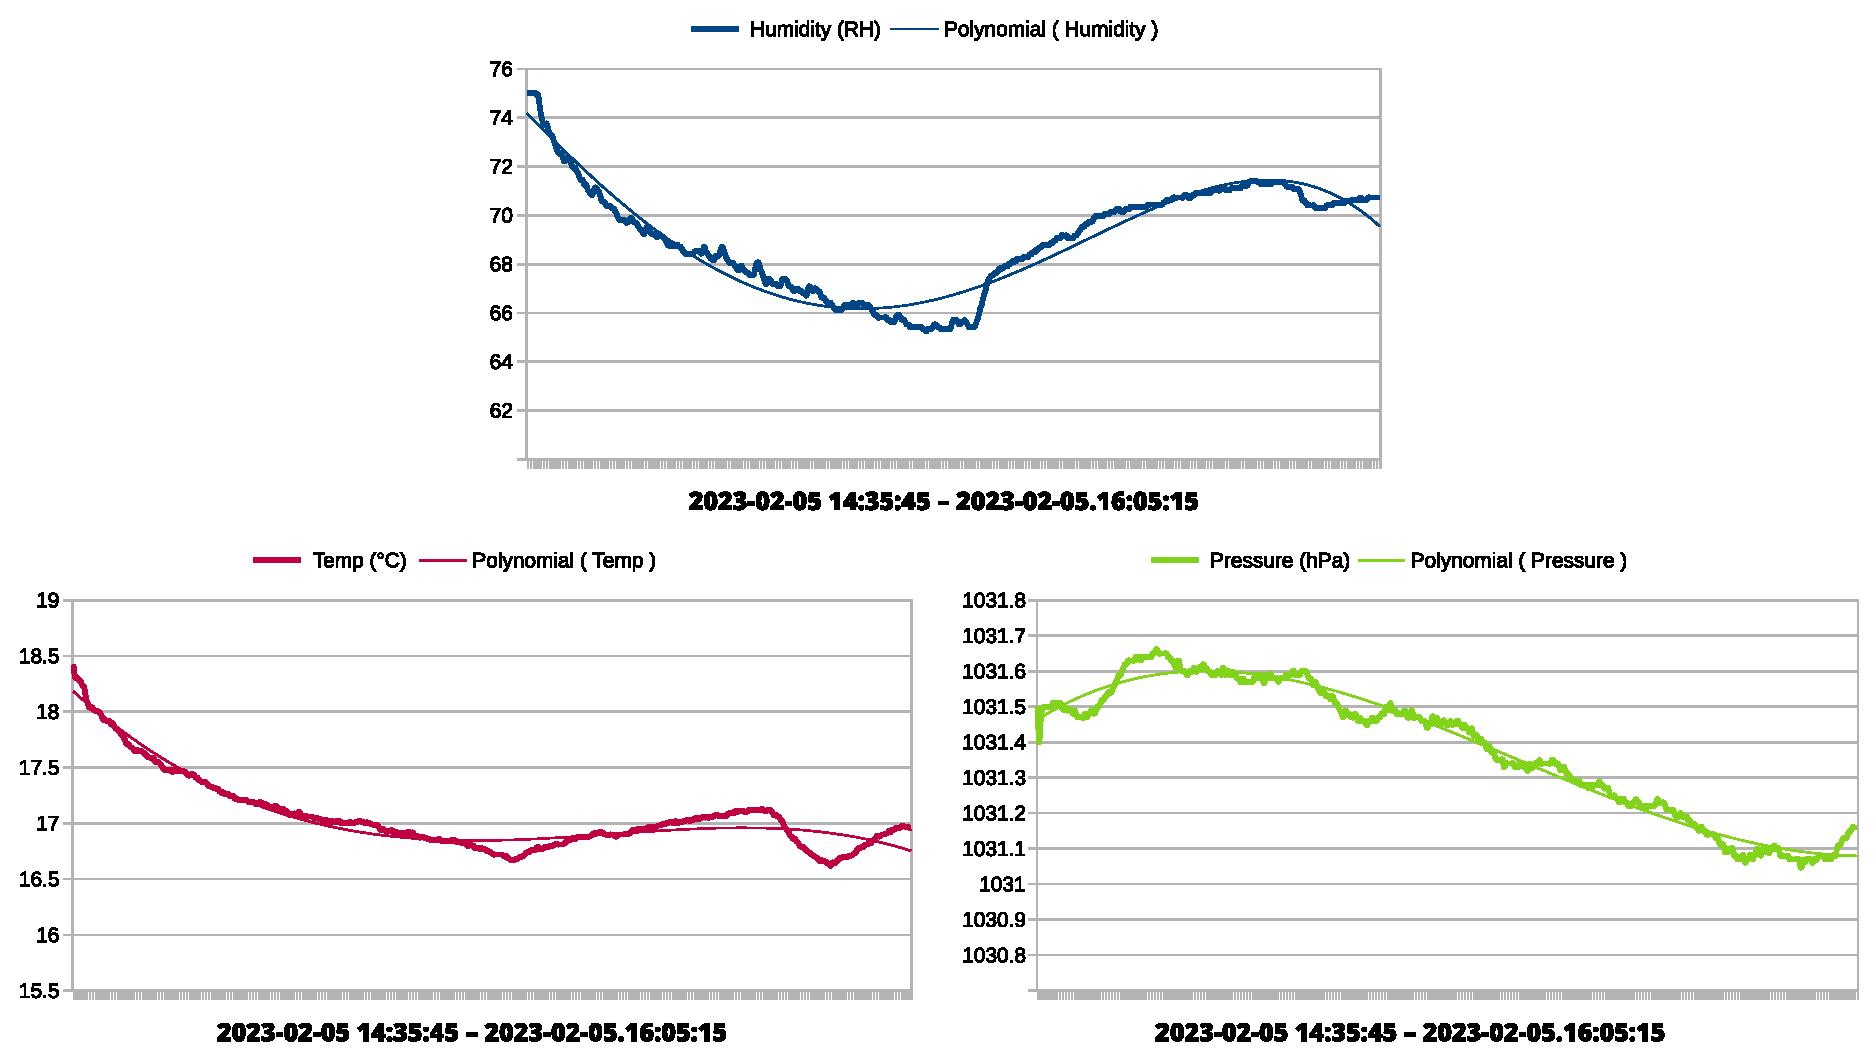
\includegraphics[width=0.5\textwidth]{media/data.pdf}
    \end{center}

    \note{
      Auswertungsbeispiel:\\~\\

      Variationen durch Öffnung eines Fensters.\\
      Luftdruck in negativer Beziehung zu Temperatur und Luftfeuchtigkeit.\\
      Sinken gehen nach Schließen des Fensters wieder zu Ausgangswerten.
    }
  \end{frame}

  \section{Epilog}%
  \subsection{Literaturverzeichnis}%
  \begin{frame}
    \printbibliography
  \end{frame}

  \subsection{Weiterführende Literatur}%
  \begin{frame}
    \note {
      Sehr empfehlenswert!
    }

    Arduino -- \href{https://docs.arduino.cc/learn/programming/sd-guide}{Guide to Arduino \& Secure Digital (SD) Storage.}~[ENG]\\
    \hspace{1em} {\footnotesize Artikel mit Beispielen zur Verwendung der SD Library}\\~\\

    Arduino -- \href{hhttps://www.arduino.cc/reference/en/libraries/sd/}{SD Library}~[ENG]\\
    \hspace{1em} {\footnotesize Dokumentation der SD Library}\\~\\

    SD Association -- \href{https://www.sdcard.org/developers/}{SD Standard Overview}~[ENG]\\
    \hspace{1em} {\footnotesize Weitere Informationen zu SD-Karten}\\~\\

    David Kriesel -- \href{https://youtu.be/\_Pd5sXXMMLI}{Big Data - mal ganz anders erklärt} \& \href{https://youtu.be/0rb9CfOvojk}{BahnMining - Pünktlichkeit ist eine Zier}\\
    \hspace{1em} {\footnotesize Beispiele interessanter Datenanalysen}\\~\\

    Dylan Beattie -- \href{https://youtu.be/gd5uJ7Nlvvo}{Plain text}~[ENG]\\
    \hspace{1em} {\footnotesize Ein Mahnruf zu den Feinheiten der Textkodierung und Lokalisierung in Computersystemen}
  \end{frame}

  \subsection{Ausklang}
  \begin{frame}[allowframebreaks, fragile]
    \vfill
      {
        \Large
        Quelltext des \textcolor{cyan}{\hyperlink{sec:project}{Beispielprogramms~Wetterstation}},
        und der \href{https://www.latex-project.org/}{\LaTeX} \href{https://ctan.org/pkg/beamer}{BEAMER} Präsentation:\\~\\
        \hspace{1em} \url{https://github.com/falco-egg/sd-presentation}
      }

      \note {
        Ende der Präsentation :3\\~\\

        Stuff ist auf GitHub.
      }
    \vfill
    {\doclicenseText \hfill \doclicenseIcon}
  \end{frame}

  \subsection*{Transflash}%
  \begin{frame}
    \fullsizegraphic{media/transflash.png}
    \note{:3 Transflash war die Bezeichung für microSD vor Namensänderung in 2005}
  \end{frame}

\end{document}
